\documentclass[11pt,a4paper]{article}
\usepackage[T1]{fontenc}
\usepackage[utf8]{inputenc}
\usepackage[margin=22mm]{geometry}
\usepackage{amsmath,amssymb}
\usepackage{siunitx}
\usepackage{booktabs}
\usepackage{graphicx}
\usepackage{tikz}
\usepackage{pgfplots}
\pgfplotsset{compat=1.17}
\usetikzlibrary{arrows.meta,positioning}
\usepackage{circuitikz}
\usepackage{listings}
\usepackage{xcolor}
\usepackage{caption}
\usepackage[hidelinks]{hyperref}

\sisetup{per-mode=symbol,detect-all}
\lstset{basicstyle=\ttfamily\scriptsize,breaklines=true,columns=fullflexible,frame=single,
  keepspaces=true,language=Python,commentstyle=\color{gray},keywordstyle=\color{blue!60!black},
  showstringspaces=false,tabsize=4}

\newcommand{\Rth}{R_{\mathrm{th}}}
\newcommand{\Zth}{Z_{\mathrm{th}}}

\title{Thermal Impedance Estimate of the Clamp Heatsink 778746\\
\large PADA profile ``G'', $225\times91$~mm section, $L=\SI{250}{\milli\metre}$, forced air cooling}
\author{D.~Bagnara}
\date{September 2026 -- Rev.~0}

\begin{document}
\maketitle

\begin{abstract}
This note estimates the heatsink-to-ambient thermal resistance and the transient thermal impedance of the clamp heatsink of drawing 778746-01-01 (\emph{Dissipatore clamp L250 225x91}), used with a press-pack thyristor having a \SI{100}{\milli\metre} contact face. The heatsink is a modular aluminium extrusion (PADA profile ``G'': 18 central modules plus two end modules) with two \SI{14}{\milli\metre} plates joined by 36 internal fins; the fins form 37 closed channels of about $4.15\times63$~mm, \SI{250}{\milli\metre} long, through which cooling air must be forced. Two independent models are used: an analytical chain (channel convection correlation, fin analysis, spreading resistance) and a three-dimensional finite-difference model that also provides the step response. For a single device on one face the estimated resistance is $\Rth\approx\SI{0.080}{\kelvin\per\watt}$ (centre of the contact face) at \SI{140}{\cubic\metre\per\hour}, decreasing to \SI{0.068}{\kelvin\per\watt} at \SI{280}{\cubic\metre\per\hour}; a design value with margin is proposed in Section~\ref{sec:summary}. A four-cell Foster network is given for transient calculations.
\end{abstract}

\section{Scope and input data}\label{sec:input}

\subsection{Data taken from the drawing}

Table~\ref{tab:drawing} lists the data read from drawing 778746-01-01 (rev.~1, 28/03/2019). Only the overall dimensions, the material, the module composition and the hole pattern are dimensioned explicitly. The internal fin geometry is drawn schematically, so fin thickness, channel width and plate thickness were scaled from the section view ($225\times91$~mm frame, 800~dpi raster); an uncertainty of about \SI{\pm 0.2}{\milli\metre} on these values must be expected and its effect is discussed in Section~\ref{sec:sens}.

\begin{table}[htbp]
\centering\small
\caption{Heatsink data. Values marked $^{*}$ are scaled from the section view.}
\label{tab:drawing}
\begin{tabular}{llr}
\toprule
Symbol & Quantity & Value \\
\midrule
 & Part / drawing no. & GR19 5000A / 778746 \\
 & Material & Al alloy for extrusion UNI~9006/1 (6060/6063) \\
 & Construction (PADA profile ``G'') & G8716 $\times1$, G8717 $\times1$, G8715 $\times18$ \\
$W$ & Width across the fins & \SI{225}{\milli\metre} \\
$H_s$ & Overall height (plate to plate) & \SI{91}{\milli\metre} \\
$L$ & Length along the channels (extrusion axis) & \SI{250}{\milli\metre} \\
$D_s$ & SCR contact area (one face, centred, $R_a\,1.2$) & \O\,\SI{100}{\milli\metre} \\
 & Clamp tie-rod holes (centre line) & $2\times$ \O\,\SI{18}{\milli\metre} through, \SI{180}{\milli\metre} apart \\
$t_b$ & Plate thickness (surface to fin root), each side$^{*}$ & \SI{14}{\milli\metre} \\
$N_f$ & Internal fins (webs)$^{*}$ & 36 \\
$t_f$ & Fin thickness$^{*}$ & \SI{1.6}{\milli\metre} \\
$b$ & Channel width$^{*}$ & \SI{4.15}{\milli\metre} \\
$p$ & Fin pitch$^{*}$ ($= t_f + b$) & \SI{5.75}{\milli\metre} \\
$N_{ch}$ & Channels$^{*}$ ($4.15\times63$~mm, rounded ends) & 37 \\
$t_w$ & Side wall thickness$^{*}$ & \SI{6.9}{\milli\metre} \\
\bottomrule
\end{tabular}
\end{table}

\begin{figure}[htbp]
\centering
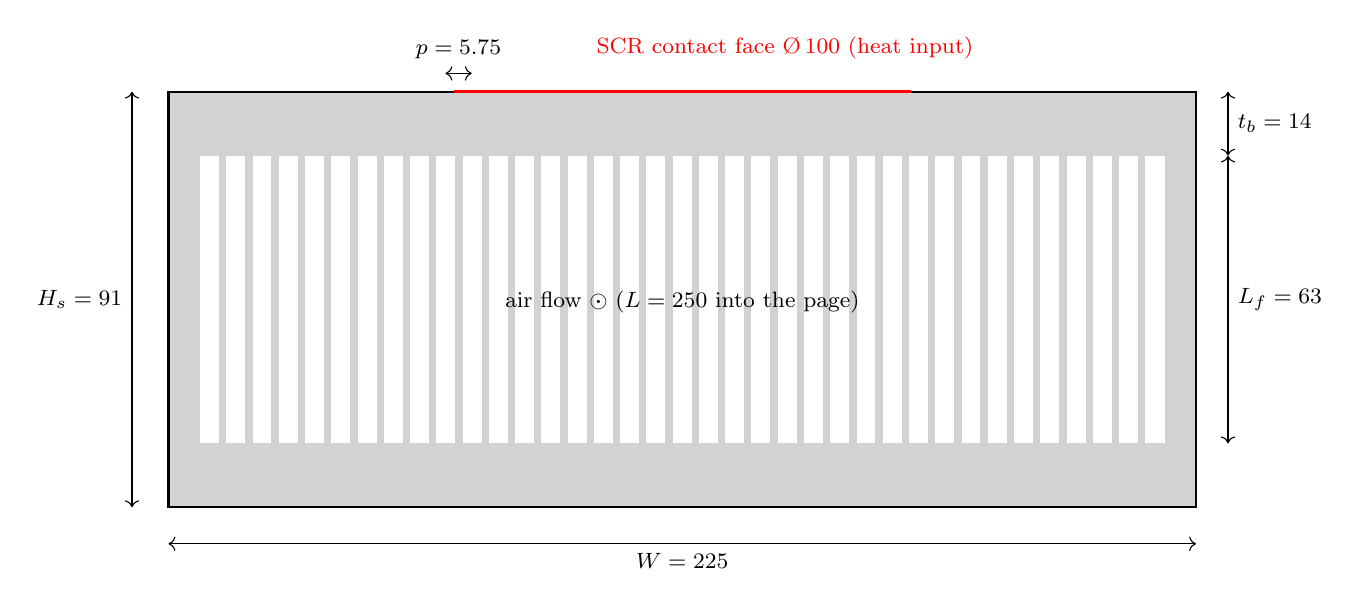
\begin{tikzpicture}[x=0.058cm,y=0.058cm]
  % plates
  \fill[gray!35] (0,0) rectangle (225,14);
  \fill[gray!35] (0,77) rectangle (225,91);
  \fill[gray!35] (0,0) rectangle (6.9,91);
  \fill[gray!35] (218.1,0) rectangle (225,91);
  \foreach \i in {0,...,35} {
    \fill[gray!35] ({11.05+\i*5.75},14) rectangle ({12.65+\i*5.75},77);
  }
  \draw[thick] (0,0) rectangle (225,91);
  % SCR contact
  \draw[red,very thick] (62.5,91) -- (162.5,91);
  \node[red,above] at (135,96) {\footnotesize SCR contact face \O\,100 (heat input)};
  % dimensions
  \draw[<->] (0,-8) -- (225,-8) node[midway,below] {\footnotesize $W=225$};
  \draw[<->] (-8,0) -- (-8,91) node[midway,left] {\footnotesize $H_s=91$};
  \draw[<->] (232,77) -- (232,91) node[midway,right] {\footnotesize $t_b=14$};
  \draw[<->] (232,14) -- (232,77) node[midway,right] {\footnotesize $L_f=63$};
  \node at (112.5,45) {\footnotesize air flow $\odot$ ($L=250$ into the page)};
  \draw[<->] (60.65,95) -- (66.4,95); \node[above] at (63.5,96) {\footnotesize $p=5.75$};
\end{tikzpicture}
\caption{Schematic cross-section used for the thermal model (dimensions in mm). The two \SI{14}{\milli\metre} plates are connected by 36 fins of \SI{1.6}{\milli\metre}; the 37 channels are closed on all four sides. The drawing shows the fin surfaces as corrugated; a smooth surface is assumed here (conservative).}
\label{fig:section}
\end{figure}

\subsection{Derived geometric quantities}

\begin{align}
L_f &= H_s - 2t_b = \SI{63}{\milli\metre} &
A_s &= \tfrac{\pi}{4}D_s^2 = \SI{7854}{\milli\metre\squared} \nonumber\\
A_p &= W L = \SI{56250}{\milli\metre\squared} &
A_s/A_p &= 0.14 \nonumber\\
A_{ff} &= N_{ch}\, b\, L_f = \SI{96.7}{\centi\metre\squared} &
\sigma &= A_{ff}/(W H_s) = 0.47 \nonumber\\
D_h &= 2 b L_f/(b+L_f) = \SI{7.8}{\milli\metre} &
A_{fin} &= 2 N_f L_f L = \SI{1.13}{\metre\squared} \nonumber
\end{align}
The exposed channel top and bottom walls add $N_{ch} b L = \SI{0.038}{\metre\squared}$ each and the inner faces of the side walls \SI{0.032}{\metre\squared}. The metal volume is about \SI{2.7}{\litre}, i.e.\ a mass of about \SI{7.3}{\kilo\gram} and a total heat capacity of about \SI{6.6}{\kilo\joule\per\kelvin}.

\subsection{Assumptions}\label{sec:assump}
\begin{enumerate}
\item Forced air enters one $225\times91$~mm face and leaves the opposite one; all channels receive the same flow (no bypass, no maldistribution). Results are given as a function of the volumetric flow $Q$ actually passing through the heatsink and of the corresponding channel velocity $V_{ch}=Q/A_{ff}$.
\item One thyristor on one face, uniform heat flux over the \O\,\SI{100}{\milli\metre} contact area. The device-to-heatsink contact resistance $\Rth(\mathrm{c\text{-}h})$ is \emph{not} included; it is taken from the device datasheet.
\item Aluminium: $k=\SI{200}{\watt\per\metre\per\kelvin}$, $\rho=\SI{2700}{\kilo\gram\per\cubic\metre}$, $c_p=\SI{900}{\joule\per\kilo\gram\per\kelvin}$. Air at \SI{40}{\celsius}: $\rho_a=\SI{1.127}{\kilo\gram\per\cubic\metre}$, $c_{p,a}=\SI{1007}{\joule\per\kilo\gram\per\kelvin}$, $k_a=\SI{0.0271}{\watt\per\metre\per\kelvin}$, $\nu_a=\SI{1.70e-5}{\metre\squared\per\second}$, $\mathrm{Pr}=0.71$.
\item Baseline: the plates are treated as monolithic. The module joints (one every two fins) are examined as a sensitivity in Section~\ref{sec:sens}.
\item Outer faces adiabatic (the second plate is not cooled from outside), radiation neglected, smooth fin surfaces, tie-rod holes neglected (they remove less than \SI{1}{\percent} of the fin surface).
\item The convection coefficient is referred to the \emph{inlet} air temperature, so that all resistances are heatsink-to-inlet-air values; the air temperature rise along the channels is embedded in the correlation of Section~\ref{sec:conv}.
\end{enumerate}

\section{Analytical steady-state model}\label{sec:analytic}

The thermal path is represented by the series of a spreading/conduction resistance in the loaded plate and a convective resistance of the fin array (Fig.~\ref{fig:network}):
\begin{equation}
\Rth(\mathrm{h\text{-}a}) = R_{sp} + \frac{1}{G}, \qquad G = N_f G_f + 2 G_w + h\,N_{ch}\,b\,L .
\label{eq:rth}
\end{equation}

\begin{figure}[htbp]
\centering
\begin{circuitikz}[american,scale=0.9,transform shape]
\draw (0,0) to[I,l=$P$] (0,2.5);
\draw (0,2.5) to[R,l=$R_{sp}$] (3,2.5) node[above]{$T_{root}$};
\draw (3,2.5) to[R,l=$1/(N_f G_f)$] (6,2.5);
\draw (3,2.5) -- (3,1) to[R,l_=$1/(2G_w)$] (6,1) -- (6,2.5);
\draw (3,2.5) -- (3,4) to[R,l=$1/(h N_{ch} b L)$] (6,4) -- (6,2.5);
\draw (6,2.5) -- (7,2.5) node[right]{$T_{air,in}$};
\draw (7,2.5) -- (7,0) -- (0,0);
\node[above] at (0,2.5) {$T_{case}$};
\end{circuitikz}
\caption{Steady-state network of Eq.~\eqref{eq:rth}: plate spreading in series with the parallel of fins, side walls and directly exposed channel top walls.}
\label{fig:network}
\end{figure}

\subsection{Channel convection coefficient}\label{sec:conv}

The channels are narrow ($b/L_f = 0.066$) and the flow is laminar over the whole practical range ($\mathrm{Re}_{D_h}<2500$ up to \SI{10}{\metre\per\second}). With $L/D_h=32$ the thermal boundary layers are still developing over a large part of the length, so neither the fully developed nor the flat-plate limit applies alone. The composite model of Teertstra, Yovanovich and Culham~\cite{teertstra1999} for parallel-plate channels is used:
\begin{equation}
\mathrm{Nu}_b = \left[\left(\frac{\mathrm{Re}_b^{*}\,\mathrm{Pr}}{2}\right)^{-3}
+ \left(0.664\sqrt{\mathrm{Re}_b^{*}}\;\mathrm{Pr}^{1/3}\sqrt{1+\frac{3.65}{\sqrt{\mathrm{Re}_b^{*}}}}\right)^{-3}\right]^{-1/3},
\qquad \mathrm{Re}_b^{*} = \frac{V_{ch} b}{\nu_a}\cdot\frac{b}{L},
\label{eq:nu}
\end{equation}
and $h = \mathrm{Nu}_b\,k_a/b$. The first term is the energy-balance limit (outlet air at wall temperature), the second the developing-flow limit; $h$ is therefore defined on the wall-to-inlet temperature difference. At $V_{ch}=\SI{4}{\metre\per\second}$ ($Q\approx\SI{140}{\cubic\metre\per\hour}$): $\mathrm{Re}_b=976$, $\mathrm{Re}_b^{*}=16$, $\mathrm{Nu}_b=3.1$, $h=\SI{20}{\watt\per\metre\squared\per\kelvin}$. The heatsink then works at about \SI{55}{\percent} of its energy-balance limit, i.e.\ the outlet air is already at roughly half of the wall-to-inlet temperature difference: increasing the flow is more effective than increasing the surface.

\subsection{Fin conductance}\label{sec:fin}

Each fin ($t_f$, length $L_f$, depth $L$) is a straight fin whose far end is attached to the second plate. The second plate is thick and nearly isothermal; it collects the fin-tip heat and releases it through the channel bottom walls. It is therefore modelled as a convective tip whose coefficient is scaled by the collector-to-cross-section area ratio, $h_t = h\,b/t_f$, giving
\begin{equation}
G_f = \sqrt{2 h k t_f}\;L\;\frac{\sinh(mL_f)+\zeta\cosh(mL_f)}{\cosh(mL_f)+\zeta\sinh(mL_f)},\qquad
m=\sqrt{\frac{2h}{k t_f}},\qquad \zeta=\frac{h_t}{mk}.
\label{eq:fin}
\end{equation}
The same expression, with one convecting face and $h_t = h\,(b/2)/t_w$, gives the side-wall conductance $G_w$. At $h=\SI{20}{\watt\per\metre\squared\per\kelvin}$: $mL_f=0.71$, adiabatic-tip efficiency $0.86$, effective efficiency including the second plate $\eta_f = G_f/(2hL_fL)=0.88$. The fins are efficient; a thicker fin would gain little.

\subsection{Spreading resistance in the loaded plate}\label{sec:spread}

The \O\,\SI{100}{\milli\metre} source covers only \SI{14}{\percent} of the $250\times225$~mm plate, and the plate (\SI{14}{\milli\metre}) is thin compared with the spreading distance, so the constriction resistance is significant. The closed-form model of Lee, Song, Au and Moran~\cite{lee1995} for a circular source of radius $a$ on a circular plate of equivalent radius $r_p=\sqrt{A_p/\pi}=\SI{133.8}{\milli\metre}$, thickness $t_b$, with a uniform effective coefficient $h_{eff}=G/A_p$ on the finned side, is used:
\begin{gather}
\varepsilon=\frac{a}{r_p},\quad \tau=\frac{t_b}{r_p},\quad \mathrm{Bi}=\frac{h_{eff}\,r_p}{k},\quad
\lambda=\pi+\frac{1}{\varepsilon\sqrt{\pi}},\quad
\Phi=\frac{\tanh(\lambda\tau)+\lambda/\mathrm{Bi}}{1+(\lambda/\mathrm{Bi})\tanh(\lambda\tau)},\nonumber\\
\psi_{max}=\frac{\varepsilon\tau}{\sqrt{\pi}}+\frac{(1-\varepsilon)\,\Phi}{\sqrt{\pi}},\qquad
\psi_{avg}=\frac{\varepsilon\tau}{\sqrt{\pi}}+\tfrac12(1-\varepsilon)^{3/2}\Phi,\qquad
R_{sp}=\frac{\psi}{k\sqrt{A_s}} .
\label{eq:lee}
\end{gather}
$\psi_{max}$ refers to the centre of the contact face, $\psi_{avg}$ to its area-averaged temperature; both include the one-dimensional conduction through the plate. At \SI{4}{\metre\per\second}: $\mathrm{Bi}=0.26$, $\Phi=2.0$, $R_{sp,max}=\SI{0.042}{\kelvin\per\watt}$, $R_{sp,avg}=\SI{0.030}{\kelvin\per\watt}$, against a convective resistance $1/G=\SI{0.046}{\kelvin\per\watt}$: the plate constriction is of the same order as the convective term and is almost independent of the flow rate. This is the main limitation of the heatsink for a \O\,\SI{100}{\milli\metre} device.

\subsection{Pressure drop}\label{sec:dp}

For fan selection the pressure drop across the heatsink is estimated with the laminar developing-flow apparent friction factor of Shah and London~\cite{shah1978} for a rectangular duct of aspect ratio $b/L_f$, plus contraction and expansion losses at the faces:
\begin{equation}
\Delta p = \tfrac12\rho_a V_{ch}^2\left[4 f_{app}\frac{L}{D_h} + K_c + K_e\right],\qquad
K_c = 0.42(1-\sigma^2),\quad K_e=(1-\sigma^2)^2 .
\label{eq:dp}
\end{equation}
Duct and plenum losses are not included.

\section{Finite-difference model}\label{sec:fd}

The analytical chain treats the plate as isotropic and the fin array as a uniform film. In reality the fins are continuous plates in the flow direction and conduct heat along $x$, the second plate spreads heat too, and the fin-root temperature is far from uniform. To check the analytical result and to obtain the step response, a three-dimensional finite-difference model was built (script in Appendix~\ref{app:fd}):
\begin{itemize}
\item loaded plate: $50\times38\times7$ cells ($\Delta x=\SI{5}{\milli\metre}$, one cell per fin pitch in $y$, $\Delta z=\SI{2}{\milli\metre}$);
\item fins and side walls: $50\times10$ cells each, conduction along $x$ and along the fin, convection on both faces (one face for the side walls);
\item second plate: $50\times38\times2$ cells, fed by the fin tips, convecting through the channel bottom walls;
\item source: uniform flux on the top layer over the cells inside the \O\,\SI{100}{\milli\metre} circle (area fractions by sub-sampling);
\item uniform $h$ from Eq.~\eqref{eq:nu}, referred to inlet air; \num{36100} unknowns.
\end{itemize}
The steady state is solved directly; the step response is integrated with the implicit Euler scheme (90 steps per decade from \SI{1}{\milli\second} to \SI{e5}{\second}). The reported case temperature is the surface value (node value plus half-cell correction), either averaged over the contact area or taken at its centre.

Figure~\ref{fig:profiles} shows the temperature distribution at \SI{140}{\cubic\metre\per\hour}. The fin-root temperature under the centre of the device is about $1.8$ times the value at the plate ends; the fins directly under the footprint (\SI{14}{\percent} of the area) convect only \SI{17.5}{\percent} of the heat, i.e.\ the plate does spread the heat, but at the cost of a large lateral temperature drop. The second plate sits at roughly half of the loaded-plate centre temperature rise: the fins work as a bridge between the two plates and the second plate contributes to the exchange.

\begin{figure}[htbp]
\centering
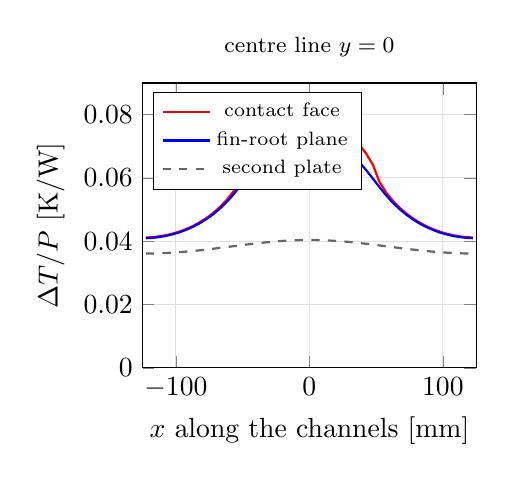
\begin{tikzpicture}
\begin{axis}[width=0.48\textwidth,height=5.2cm,xlabel={$x$ along the channels [mm]},ylabel={$\Delta T/P$ [K/W]},
  grid=both,grid style={gray!25},legend style={font=\scriptsize,at={(0.03,0.97)},anchor=north west},
  scaled y ticks=false,yticklabel style={/pgf/number format/fixed,/pgf/number format/precision=2},ymin=0,ymax=0.09,xmin=-125,xmax=125,title={\footnotesize centre line $y=0$}]
\addplot[red,thick] table[x index=0,y index=1] {
-122.5 0.04117 0.04096 0.03610
-117.5 0.04129 0.04107 0.03613
-112.5 0.04153 0.04131 0.03619
-107.5 0.04190 0.04168 0.03628
-102.5 0.04240 0.04217 0.03640
-97.5 0.04304 0.04279 0.03654
-92.5 0.04382 0.04357 0.03671
-87.5 0.04477 0.04450 0.03691
-82.5 0.04590 0.04560 0.03712
-77.5 0.04723 0.04689 0.03736
-72.5 0.04879 0.04840 0.03761
-67.5 0.05062 0.05015 0.03787
-62.5 0.05279 0.05217 0.03813
-57.5 0.05540 0.05448 0.03840
-52.5 0.05871 0.05706 0.03867
-47.5 0.06420 0.05981 0.03894
-42.5 0.06768 0.06247 0.03919
-37.5 0.07050 0.06491 0.03943
-32.5 0.07284 0.06705 0.03965
-27.5 0.07479 0.06888 0.03985
-22.5 0.07637 0.07039 0.04002
-17.5 0.07763 0.07159 0.04016
-12.5 0.07856 0.07248 0.04027
-7.5 0.07917 0.07307 0.04034
-2.5 0.07948 0.07337 0.04038
2.5 0.07948 0.07337 0.04038
7.5 0.07917 0.07307 0.04034
12.5 0.07856 0.07248 0.04027
17.5 0.07763 0.07159 0.04016
22.5 0.07637 0.07039 0.04002
27.5 0.07479 0.06888 0.03985
32.5 0.07284 0.06705 0.03965
37.5 0.07050 0.06491 0.03943
42.5 0.06768 0.06247 0.03919
47.5 0.06420 0.05981 0.03894
52.5 0.05871 0.05706 0.03867
57.5 0.05540 0.05448 0.03840
62.5 0.05279 0.05217 0.03813
67.5 0.05062 0.05015 0.03787
72.5 0.04879 0.04840 0.03761
77.5 0.04723 0.04689 0.03736
82.5 0.04590 0.04560 0.03712
87.5 0.04477 0.04450 0.03691
92.5 0.04382 0.04357 0.03671
97.5 0.04304 0.04279 0.03654
102.5 0.04240 0.04217 0.03640
107.5 0.04190 0.04168 0.03628
112.5 0.04153 0.04131 0.03619
117.5 0.04129 0.04107 0.03613
122.5 0.04117 0.04096 0.03610
};
\addplot[blue,thick] table[x index=0,y index=2] {
-122.5 0.04117 0.04096 0.03610
-117.5 0.04129 0.04107 0.03613
-112.5 0.04153 0.04131 0.03619
-107.5 0.04190 0.04168 0.03628
-102.5 0.04240 0.04217 0.03640
-97.5 0.04304 0.04279 0.03654
-92.5 0.04382 0.04357 0.03671
-87.5 0.04477 0.04450 0.03691
-82.5 0.04590 0.04560 0.03712
-77.5 0.04723 0.04689 0.03736
-72.5 0.04879 0.04840 0.03761
-67.5 0.05062 0.05015 0.03787
-62.5 0.05279 0.05217 0.03813
-57.5 0.05540 0.05448 0.03840
-52.5 0.05871 0.05706 0.03867
-47.5 0.06420 0.05981 0.03894
-42.5 0.06768 0.06247 0.03919
-37.5 0.07050 0.06491 0.03943
-32.5 0.07284 0.06705 0.03965
-27.5 0.07479 0.06888 0.03985
-22.5 0.07637 0.07039 0.04002
-17.5 0.07763 0.07159 0.04016
-12.5 0.07856 0.07248 0.04027
-7.5 0.07917 0.07307 0.04034
-2.5 0.07948 0.07337 0.04038
2.5 0.07948 0.07337 0.04038
7.5 0.07917 0.07307 0.04034
12.5 0.07856 0.07248 0.04027
17.5 0.07763 0.07159 0.04016
22.5 0.07637 0.07039 0.04002
27.5 0.07479 0.06888 0.03985
32.5 0.07284 0.06705 0.03965
37.5 0.07050 0.06491 0.03943
42.5 0.06768 0.06247 0.03919
47.5 0.06420 0.05981 0.03894
52.5 0.05871 0.05706 0.03867
57.5 0.05540 0.05448 0.03840
62.5 0.05279 0.05217 0.03813
67.5 0.05062 0.05015 0.03787
72.5 0.04879 0.04840 0.03761
77.5 0.04723 0.04689 0.03736
82.5 0.04590 0.04560 0.03712
87.5 0.04477 0.04450 0.03691
92.5 0.04382 0.04357 0.03671
97.5 0.04304 0.04279 0.03654
102.5 0.04240 0.04217 0.03640
107.5 0.04190 0.04168 0.03628
112.5 0.04153 0.04131 0.03619
117.5 0.04129 0.04107 0.03613
122.5 0.04117 0.04096 0.03610
};
\addplot[black!60,thick,dashed] table[x index=0,y index=3] {
-122.5 0.04117 0.04096 0.03610
-117.5 0.04129 0.04107 0.03613
-112.5 0.04153 0.04131 0.03619
-107.5 0.04190 0.04168 0.03628
-102.5 0.04240 0.04217 0.03640
-97.5 0.04304 0.04279 0.03654
-92.5 0.04382 0.04357 0.03671
-87.5 0.04477 0.04450 0.03691
-82.5 0.04590 0.04560 0.03712
-77.5 0.04723 0.04689 0.03736
-72.5 0.04879 0.04840 0.03761
-67.5 0.05062 0.05015 0.03787
-62.5 0.05279 0.05217 0.03813
-57.5 0.05540 0.05448 0.03840
-52.5 0.05871 0.05706 0.03867
-47.5 0.06420 0.05981 0.03894
-42.5 0.06768 0.06247 0.03919
-37.5 0.07050 0.06491 0.03943
-32.5 0.07284 0.06705 0.03965
-27.5 0.07479 0.06888 0.03985
-22.5 0.07637 0.07039 0.04002
-17.5 0.07763 0.07159 0.04016
-12.5 0.07856 0.07248 0.04027
-7.5 0.07917 0.07307 0.04034
-2.5 0.07948 0.07337 0.04038
2.5 0.07948 0.07337 0.04038
7.5 0.07917 0.07307 0.04034
12.5 0.07856 0.07248 0.04027
17.5 0.07763 0.07159 0.04016
22.5 0.07637 0.07039 0.04002
27.5 0.07479 0.06888 0.03985
32.5 0.07284 0.06705 0.03965
37.5 0.07050 0.06491 0.03943
42.5 0.06768 0.06247 0.03919
47.5 0.06420 0.05981 0.03894
52.5 0.05871 0.05706 0.03867
57.5 0.05540 0.05448 0.03840
62.5 0.05279 0.05217 0.03813
67.5 0.05062 0.05015 0.03787
72.5 0.04879 0.04840 0.03761
77.5 0.04723 0.04689 0.03736
82.5 0.04590 0.04560 0.03712
87.5 0.04477 0.04450 0.03691
92.5 0.04382 0.04357 0.03671
97.5 0.04304 0.04279 0.03654
102.5 0.04240 0.04217 0.03640
107.5 0.04190 0.04168 0.03628
112.5 0.04153 0.04131 0.03619
117.5 0.04129 0.04107 0.03613
122.5 0.04117 0.04096 0.03610
};
\legend{contact face,fin-root plane,second plate}
\end{axis}
\end{tikzpicture}\hfill
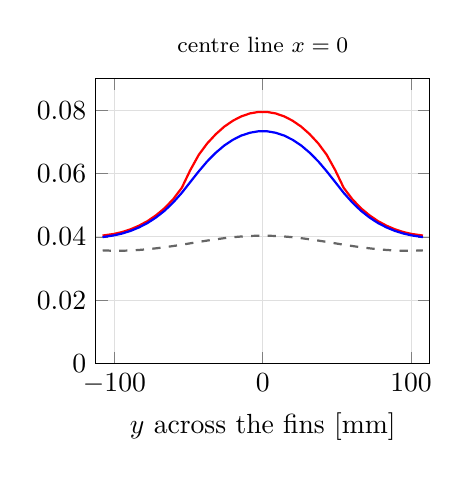
\begin{tikzpicture}
\begin{axis}[width=0.48\textwidth,height=5.2cm,xlabel={$y$ across the fins [mm]},
  grid=both,grid style={gray!25},scaled y ticks=false,yticklabel style={/pgf/number format/fixed,/pgf/number format/precision=2},ymin=0,ymax=0.09,xmin=-112.5,xmax=112.5,title={\footnotesize centre line $x=0$}]
\addplot[red,thick] table[x index=0,y index=1] {
-108.0 0.04043 0.03994 0.03575
-100.6 0.04092 0.04046 0.03562
-94.9 0.04153 0.04106 0.03563
-89.1 0.04241 0.04190 0.03572
-83.4 0.04356 0.04301 0.03588
-77.6 0.04502 0.04441 0.03611
-71.9 0.04685 0.04616 0.03640
-66.1 0.04910 0.04830 0.03674
-60.4 0.05191 0.05087 0.03712
-54.6 0.05549 0.05391 0.03754
-48.9 0.06106 0.05731 0.03798
-43.1 0.06596 0.06074 0.03842
-37.4 0.06956 0.06389 0.03885
-31.6 0.07248 0.06662 0.03925
-25.9 0.07485 0.06889 0.03961
-20.1 0.07672 0.07069 0.03991
-14.4 0.07810 0.07203 0.04014
-8.6 0.07902 0.07292 0.04030
-2.9 0.07948 0.07337 0.04038
2.9 0.07948 0.07337 0.04038
8.6 0.07902 0.07292 0.04030
14.4 0.07810 0.07203 0.04014
20.1 0.07672 0.07069 0.03991
25.9 0.07485 0.06889 0.03961
31.6 0.07248 0.06662 0.03925
37.4 0.06956 0.06389 0.03885
43.1 0.06596 0.06074 0.03842
48.9 0.06106 0.05731 0.03798
54.6 0.05549 0.05391 0.03754
60.4 0.05191 0.05087 0.03712
66.1 0.04910 0.04830 0.03674
71.9 0.04685 0.04616 0.03640
77.6 0.04502 0.04441 0.03611
83.4 0.04356 0.04301 0.03588
89.1 0.04241 0.04190 0.03572
94.9 0.04153 0.04106 0.03563
100.6 0.04092 0.04046 0.03562
108.0 0.04043 0.03994 0.03575
};
\addplot[blue,thick] table[x index=0,y index=2] {
-108.0 0.04043 0.03994 0.03575
-100.6 0.04092 0.04046 0.03562
-94.9 0.04153 0.04106 0.03563
-89.1 0.04241 0.04190 0.03572
-83.4 0.04356 0.04301 0.03588
-77.6 0.04502 0.04441 0.03611
-71.9 0.04685 0.04616 0.03640
-66.1 0.04910 0.04830 0.03674
-60.4 0.05191 0.05087 0.03712
-54.6 0.05549 0.05391 0.03754
-48.9 0.06106 0.05731 0.03798
-43.1 0.06596 0.06074 0.03842
-37.4 0.06956 0.06389 0.03885
-31.6 0.07248 0.06662 0.03925
-25.9 0.07485 0.06889 0.03961
-20.1 0.07672 0.07069 0.03991
-14.4 0.07810 0.07203 0.04014
-8.6 0.07902 0.07292 0.04030
-2.9 0.07948 0.07337 0.04038
2.9 0.07948 0.07337 0.04038
8.6 0.07902 0.07292 0.04030
14.4 0.07810 0.07203 0.04014
20.1 0.07672 0.07069 0.03991
25.9 0.07485 0.06889 0.03961
31.6 0.07248 0.06662 0.03925
37.4 0.06956 0.06389 0.03885
43.1 0.06596 0.06074 0.03842
48.9 0.06106 0.05731 0.03798
54.6 0.05549 0.05391 0.03754
60.4 0.05191 0.05087 0.03712
66.1 0.04910 0.04830 0.03674
71.9 0.04685 0.04616 0.03640
77.6 0.04502 0.04441 0.03611
83.4 0.04356 0.04301 0.03588
89.1 0.04241 0.04190 0.03572
94.9 0.04153 0.04106 0.03563
100.6 0.04092 0.04046 0.03562
108.0 0.04043 0.03994 0.03575
};
\addplot[black!60,thick,dashed] table[x index=0,y index=3] {
-108.0 0.04043 0.03994 0.03575
-100.6 0.04092 0.04046 0.03562
-94.9 0.04153 0.04106 0.03563
-89.1 0.04241 0.04190 0.03572
-83.4 0.04356 0.04301 0.03588
-77.6 0.04502 0.04441 0.03611
-71.9 0.04685 0.04616 0.03640
-66.1 0.04910 0.04830 0.03674
-60.4 0.05191 0.05087 0.03712
-54.6 0.05549 0.05391 0.03754
-48.9 0.06106 0.05731 0.03798
-43.1 0.06596 0.06074 0.03842
-37.4 0.06956 0.06389 0.03885
-31.6 0.07248 0.06662 0.03925
-25.9 0.07485 0.06889 0.03961
-20.1 0.07672 0.07069 0.03991
-14.4 0.07810 0.07203 0.04014
-8.6 0.07902 0.07292 0.04030
-2.9 0.07948 0.07337 0.04038
2.9 0.07948 0.07337 0.04038
8.6 0.07902 0.07292 0.04030
14.4 0.07810 0.07203 0.04014
20.1 0.07672 0.07069 0.03991
25.9 0.07485 0.06889 0.03961
31.6 0.07248 0.06662 0.03925
37.4 0.06956 0.06389 0.03885
43.1 0.06596 0.06074 0.03842
48.9 0.06106 0.05731 0.03798
54.6 0.05549 0.05391 0.03754
60.4 0.05191 0.05087 0.03712
66.1 0.04910 0.04830 0.03674
71.9 0.04685 0.04616 0.03640
77.6 0.04502 0.04441 0.03611
83.4 0.04356 0.04301 0.03588
89.1 0.04241 0.04190 0.03572
94.9 0.04153 0.04106 0.03563
100.6 0.04092 0.04046 0.03562
108.0 0.04043 0.03994 0.03575
};
\end{axis}
\end{tikzpicture}
\caption{Steady-state temperature rise above inlet air per watt (finite-difference model, $Q=\SI{139}{\cubic\metre\per\hour}$, $V_{ch}=\SI{4}{\metre\per\second}$). The source extends over $|x|,|y|<\SI{50}{\milli\metre}$.}
\label{fig:profiles}
\end{figure}

\section{Steady-state results}\label{sec:results}

Table~\ref{tab:sweep} and Fig.~\ref{fig:rth} give the results of both models as a function of the flow through the heatsink. The finite-difference values are \SIrange{6}{10}{\percent} lower than the analytical ones because of the additional spreading through the fins and the second plate; the agreement supports both estimates. The finite-difference value referred to the centre of the contact face, $\Rth^{max}$, is the recommended basis since the case temperature of a press-pack device is normally checked at the centre of the pole face; $\Rth^{avg}$ is the area-averaged value.

\begin{table}[htbp]
\centering\scriptsize
\setlength{\tabcolsep}{3.5pt}
\caption{Heatsink-to-inlet-air resistance versus flow. $Q$: flow through the heatsink; $V_{ch}$: channel velocity; $\eta_f$: effective fin efficiency; $G$: total conductance of the fin array; $R_{sp}$: plate spreading (Eq.~\ref{eq:lee}); ``an.'': Eq.~\eqref{eq:rth}; ``FD'': finite-difference model; $\Delta p$: Eq.~\eqref{eq:dp}. Resistances in \si{\kelvin\per\watt}.}
\label{tab:sweep}
\begin{tabular}{rrrrrrrrrrrrrrr}
\toprule
$Q$ & $V_{ch}$ & $\mathrm{Re}_b$ & $\mathrm{Nu}_b$ & $h$ & $\eta_f$ & $G$ & $1/G$ & $R_{sp}^{avg}$ & $R_{sp}^{max}$ & $\Rth^{avg}$ & $\Rth^{max}$ & $\Rth^{avg}$ & $\Rth^{max}$ & $\Delta p$ \\
\si{\cubic\metre\per\hour} & \si{\metre\per\second} & & & \si{\watt\per\metre\squared\per\kelvin} & & \si{\watt\per\kelvin} & & & & an. & an. & FD & FD & \si{\pascal} \\
\midrule
35 & 1.0 & 244 & 1.29 & 8.5 & 0.962 & 9.8 & 0.1018 & 0.0309 & 0.0435 & 0.1327 & 0.1454 & 0.1270 & 0.1358 & 4 \\
52 & 1.5 & 366 & 1.77 & 11.5 & 0.939 & 13.1 & 0.0764 & 0.0305 & 0.0430 & 0.1069 & 0.1193 & 0.1015 & 0.1102 & 7 \\
70 & 2.0 & 488 & 2.14 & 14.0 & 0.922 & 15.6 & 0.0642 & 0.0302 & 0.0425 & 0.0944 & 0.1067 & 0.0892 & 0.0979 & 11 \\
87 & 2.5 & 610 & 2.44 & 15.9 & 0.909 & 17.5 & 0.0570 & 0.0300 & 0.0422 & 0.0870 & 0.0993 & 0.0820 & 0.0906 & 14 \\
104 & 3.0 & 732 & 2.69 & 17.6 & 0.898 & 19.1 & 0.0522 & 0.0298 & 0.0420 & 0.0820 & 0.0942 & 0.0771 & 0.0858 & 18 \\
139 & 4.0 & 976 & 3.11 & 20.3 & 0.881 & 21.7 & 0.0461 & 0.0295 & 0.0415 & 0.0756 & 0.0876 & 0.0708 & 0.0795 & 28 \\
174 & 5.0 & 1221 & 3.45 & 22.5 & 0.867 & 23.7 & 0.0421 & 0.0293 & 0.0412 & 0.0714 & 0.0834 & 0.0668 & 0.0754 & 39 \\
209 & 6.0 & 1465 & 3.75 & 24.5 & 0.856 & 25.5 & 0.0393 & 0.0291 & 0.0410 & 0.0684 & 0.0803 & 0.0639 & 0.0725 & 53 \\
244 & 7.0 & 1709 & 4.01 & 26.2 & 0.846 & 26.9 & 0.0371 & 0.0289 & 0.0407 & 0.0661 & 0.0779 & 0.0617 & 0.0702 & 68 \\
279 & 8.0 & 1953 & 4.25 & 27.7 & 0.837 & 28.3 & 0.0354 & 0.0288 & 0.0405 & 0.0642 & 0.0759 & 0.0599 & 0.0684 & 84 \\
348 & 10.0 & 2441 & 4.68 & 30.5 & 0.822 & 30.6 & 0.0327 & 0.0286 & 0.0402 & 0.0612 & 0.0729 & 0.0571 & 0.0656 & 122 \\
\bottomrule
\end{tabular}
\end{table}

\begin{figure}[htbp]
\centering
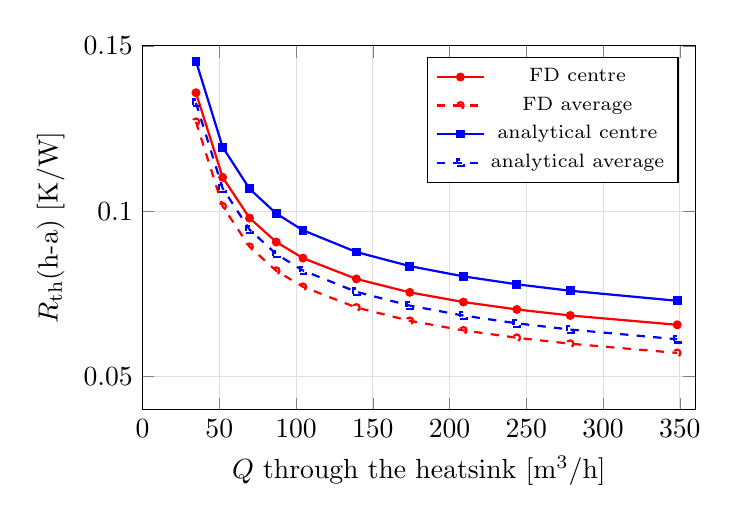
\begin{tikzpicture}
\begin{axis}[width=8.6cm,height=6.2cm,xlabel={$Q$ through the heatsink [m$^3$/h]},ylabel={$\Rth(\mathrm{h\text{-}a})$ [K/W]},
  grid=both,grid style={gray!25},xmin=0,xmax=360,ymin=0.04,ymax=0.15,scaled y ticks=false,yticklabel style={/pgf/number format/fixed,/pgf/number format/precision=2},
  legend style={font=\scriptsize,at={(0.97,0.97)},anchor=north east}]
\addplot[red,thick,mark=*,mark size=1.2pt] table[x index=0,y index=4] {
34.8 0.13273 0.14536 0.12701 0.13580 4.38 1.0
52.2 0.10688 0.11934 0.10145 0.11020 7.23 1.5
69.7 0.09441 0.10675 0.08920 0.09791 10.52 2.0
87.1 0.08702 0.09926 0.08196 0.09065 14.25 2.5
104.5 0.08204 0.09420 0.07711 0.08578 18.42 3.0
139.3 0.07558 0.08762 0.07084 0.07948 28.08 4.0
174.1 0.07141 0.08336 0.06682 0.07542 39.50 5.0
209.0 0.06840 0.08026 0.06392 0.07250 52.66 6.0
243.8 0.06606 0.07786 0.06169 0.07025 67.55 7.0
278.6 0.06417 0.07591 0.05989 0.06843 84.13 8.0
348.3 0.06124 0.07287 0.05710 0.06561 122.27 10.0
};
\addplot[red,thick,dashed,mark=o,mark size=1.2pt] table[x index=0,y index=3] {
34.8 0.13273 0.14536 0.12701 0.13580 4.38 1.0
52.2 0.10688 0.11934 0.10145 0.11020 7.23 1.5
69.7 0.09441 0.10675 0.08920 0.09791 10.52 2.0
87.1 0.08702 0.09926 0.08196 0.09065 14.25 2.5
104.5 0.08204 0.09420 0.07711 0.08578 18.42 3.0
139.3 0.07558 0.08762 0.07084 0.07948 28.08 4.0
174.1 0.07141 0.08336 0.06682 0.07542 39.50 5.0
209.0 0.06840 0.08026 0.06392 0.07250 52.66 6.0
243.8 0.06606 0.07786 0.06169 0.07025 67.55 7.0
278.6 0.06417 0.07591 0.05989 0.06843 84.13 8.0
348.3 0.06124 0.07287 0.05710 0.06561 122.27 10.0
};
\addplot[blue,thick,mark=square*,mark size=1.2pt] table[x index=0,y index=2] {
34.8 0.13273 0.14536 0.12701 0.13580 4.38 1.0
52.2 0.10688 0.11934 0.10145 0.11020 7.23 1.5
69.7 0.09441 0.10675 0.08920 0.09791 10.52 2.0
87.1 0.08702 0.09926 0.08196 0.09065 14.25 2.5
104.5 0.08204 0.09420 0.07711 0.08578 18.42 3.0
139.3 0.07558 0.08762 0.07084 0.07948 28.08 4.0
174.1 0.07141 0.08336 0.06682 0.07542 39.50 5.0
209.0 0.06840 0.08026 0.06392 0.07250 52.66 6.0
243.8 0.06606 0.07786 0.06169 0.07025 67.55 7.0
278.6 0.06417 0.07591 0.05989 0.06843 84.13 8.0
348.3 0.06124 0.07287 0.05710 0.06561 122.27 10.0
};
\addplot[blue,thick,dashed,mark=square,mark size=1.2pt] table[x index=0,y index=1] {
34.8 0.13273 0.14536 0.12701 0.13580 4.38 1.0
52.2 0.10688 0.11934 0.10145 0.11020 7.23 1.5
69.7 0.09441 0.10675 0.08920 0.09791 10.52 2.0
87.1 0.08702 0.09926 0.08196 0.09065 14.25 2.5
104.5 0.08204 0.09420 0.07711 0.08578 18.42 3.0
139.3 0.07558 0.08762 0.07084 0.07948 28.08 4.0
174.1 0.07141 0.08336 0.06682 0.07542 39.50 5.0
209.0 0.06840 0.08026 0.06392 0.07250 52.66 6.0
243.8 0.06606 0.07786 0.06169 0.07025 67.55 7.0
278.6 0.06417 0.07591 0.05989 0.06843 84.13 8.0
348.3 0.06124 0.07287 0.05710 0.06561 122.27 10.0
};
\legend{FD centre,FD average,analytical centre,analytical average}
\end{axis}
\end{tikzpicture}\hfill
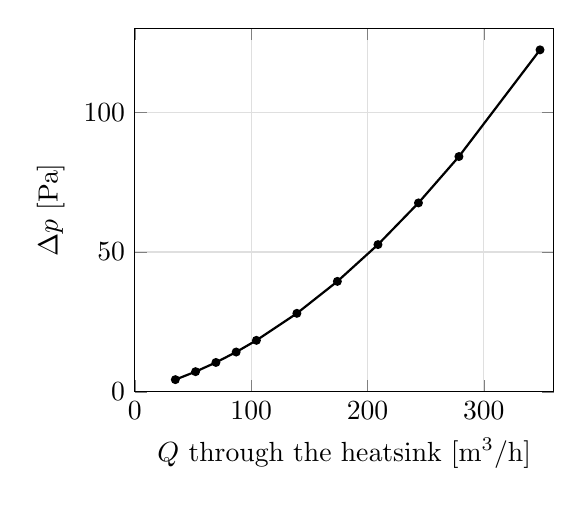
\begin{tikzpicture}
\begin{axis}[width=6.9cm,height=6.2cm,xlabel={$Q$ through the heatsink [m$^3$/h]},ylabel={$\Delta p$ [Pa]},
  grid=both,grid style={gray!25},xmin=0,xmax=360,ymin=0,ymax=130]
\addplot[black,thick,mark=*,mark size=1.2pt] table[x index=0,y index=5] {
34.8 0.13273 0.14536 0.12701 0.13580 4.38 1.0
52.2 0.10688 0.11934 0.10145 0.11020 7.23 1.5
69.7 0.09441 0.10675 0.08920 0.09791 10.52 2.0
87.1 0.08702 0.09926 0.08196 0.09065 14.25 2.5
104.5 0.08204 0.09420 0.07711 0.08578 18.42 3.0
139.3 0.07558 0.08762 0.07084 0.07948 28.08 4.0
174.1 0.07141 0.08336 0.06682 0.07542 39.50 5.0
209.0 0.06840 0.08026 0.06392 0.07250 52.66 6.0
243.8 0.06606 0.07786 0.06169 0.07025 67.55 7.0
278.6 0.06417 0.07591 0.05989 0.06843 84.13 8.0
348.3 0.06124 0.07287 0.05710 0.06561 122.27 10.0
};
\end{axis}
\end{tikzpicture}
\caption{Left: heatsink-to-inlet-air resistance versus flow. Right: estimated pressure drop across the heatsink (channels only).}
\label{fig:rth}
\end{figure}

For quick use, the finite-difference results are fitted within \SI{1.5}{\percent} over \SIrange{35}{350}{\cubic\metre\per\hour} by
\begin{equation}
\Rth^{max}(\mathrm{h\text{-}a}) \approx 0.057 + 2.14\,Q^{-0.93},\qquad
\Rth^{avg}(\mathrm{h\text{-}a}) \approx 0.049 + 2.17\,Q^{-0.94}\qquad
[\si{\kelvin\per\watt},\ Q\ \text{in}\ \si{\cubic\metre\per\hour}] .
\label{eq:fit}
\end{equation}
The constant term is essentially the plate spreading resistance: even with unlimited flow the resistance would not fall below about \SI{0.05}{\kelvin\per\watt}, which sets the useful range of this heatsink with a \O\,\SI{100}{\milli\metre} device.

\section{Sensitivity and uncertainty}\label{sec:sens}

\paragraph{Module joints.} The plates are built from 20 interlocked modules; in the finite-difference model a contact conductance $h_j$ was inserted at every module boundary (every two fins) across the full plate thickness, Table~\ref{tab:joint}. Pressed aluminium-to-aluminium joints typically lie between \SIlist{10;50}{\kilo\watt\per\metre\squared\per\kelvin}; the hooked interface has about twice the area of a plane cut, which partly compensates. An increase of \SIrange{5}{15}{\percent} of the resistance with respect to the monolithic case should be expected unless the modules are bonded.

\begin{table}[htbp]
\centering\small
\caption{Effect of the module joint conductance at $Q=\SI{139}{\cubic\metre\per\hour}$ (FD model).}
\label{tab:joint}
\begin{tabular}{lrrrr}
\toprule
$h_j$ [\si{\kilo\watt\per\metre\squared\per\kelvin}] & $\Rth^{avg}$ & $\Rth^{max}$ & $\Delta\Rth^{avg}$ & $\Delta\Rth^{max}$ \\
\midrule
$\infty$ (monolithic) & 0.0708 & 0.0795 & +0\,\% & +0\,\% \\
50 & 0.0734 & 0.0830 & +4\,\% & +4\,\% \\
20 & 0.0765 & 0.0873 & +8\,\% & +10\,\% \\
10 & 0.0806 & 0.0929 & +14\,\% & +17\,\% \\
5 & 0.0866 & 0.1010 & +22\,\% & +27\,\% \\
\bottomrule
\end{tabular}
\end{table}

\paragraph{Other parameters (at \SI{139}{\cubic\metre\per\hour}).}
\begin{itemize}
\item Aluminium conductivity \SI{170}{\watt\per\metre\per\kelvin} instead of 200 (e.g.\ 6082 or poorly tempered 6060): $+8\,\%$ on $\Rth^{max}$.
\item Fin thickness \SI{1.4}{\milli\metre} instead of 1.6: $\eta_f$ drops from 0.88 to 0.87, effect below \SI{2}{\percent}. Channel width \SI{\pm 0.2}{\milli\metre}: changes $V_{ch}$ at constant $Q$ by \SI{\pm 5}{\percent}, effect on $\Rth$ about \SI{\pm 2}{\percent}.
\item Natural convection (\SI{5}{\watt\per\metre\squared\per\kelvin}) on the free face of the second plate and on the side walls: $\Rth^{avg}=\SI{0.0703}{\kelvin\per\watt}$, $\Rth^{max}=\SI{0.0789}{\kelvin\per\watt}$, i.e.\ less than \SI{1}{\percent} gain; the outer faces do not matter.
\item Corrugated fin surfaces, as suggested by the drawing, would increase $h$ by typically \SIrange{20}{40}{\percent} in this laminar regime; since half of the resistance is in the plate, the gain on $\Rth$ would be limited to \SIrange{8}{15}{\percent}. It is not credited here.
\item Flow maldistribution or bypass around the heatsink reduce the effective $Q$; Eq.~\eqref{eq:fit} should be entered with the flow actually passing through the channels.
\end{itemize}

\paragraph{Overall.} Correlation-based estimates of this kind are usually within \SI{\pm 15}{\percent} of measurements. Combining this with the joint effect, a design margin of \SI{15}{\percent} on the monolithic finite-difference value is suggested.

\paragraph{Natural convection.} With the channels vertical (Elenbaas correlation~\cite{elenbaas1942}, $\Delta T=\SI{50}{\kelvin}$) the channel coefficient would be only about \SI{1.2}{\watt\per\metre\squared\per\kelvin} because of the \SI{4}{\milli\metre} gap; including the outer faces the resistance would be of the order of \SIrange{0.4}{0.6}{\kelvin\per\watt}. The heatsink is not meant for natural convection.

\section{Transient thermal impedance}\label{sec:transient}

Figure~\ref{fig:zth} shows the step response of the finite-difference model for three flow rates; Table~\ref{tab:zth} lists selected values. Up to about \SI{30}{\second} the impedance is independent of the flow (within \SI{1.5}{\percent}) and up to \SI{100}{\second} within \SI{5}{\percent}: overload calculations in this range do not depend on the fan operating point. The steady state is reached after about one hour ($\tau\approx\SIrange{170}{370}{\second}$ for the last cell, set by the \SI{6.6}{\kilo\joule\per\kelvin} of the aluminium).

For $t<\SI{0.1}{\second}$ the mesh resolution (\SI{2}{\milli\metre} layers) is not sufficient; there the semi-infinite-body solution applies,
\begin{equation}
\Zth(t) \approx \frac{2}{k A_s}\sqrt{\frac{\alpha t}{\pi}},\qquad \alpha=\frac{k}{\rho c_p}=\SI{8.2e-5}{\metre\squared\per\second},
\label{eq:semi}
\end{equation}
which gives \SI{0.65e-3}{\kelvin\per\watt} at \SI{10}{\milli\second} and matches the model from \SI{0.1}{\second} on (dotted line in Fig.~\ref{fig:zth}). In this range the heatsink contribution is negligible compared with the junction-to-case impedance of the device.

\begin{figure}[htbp]
\centering
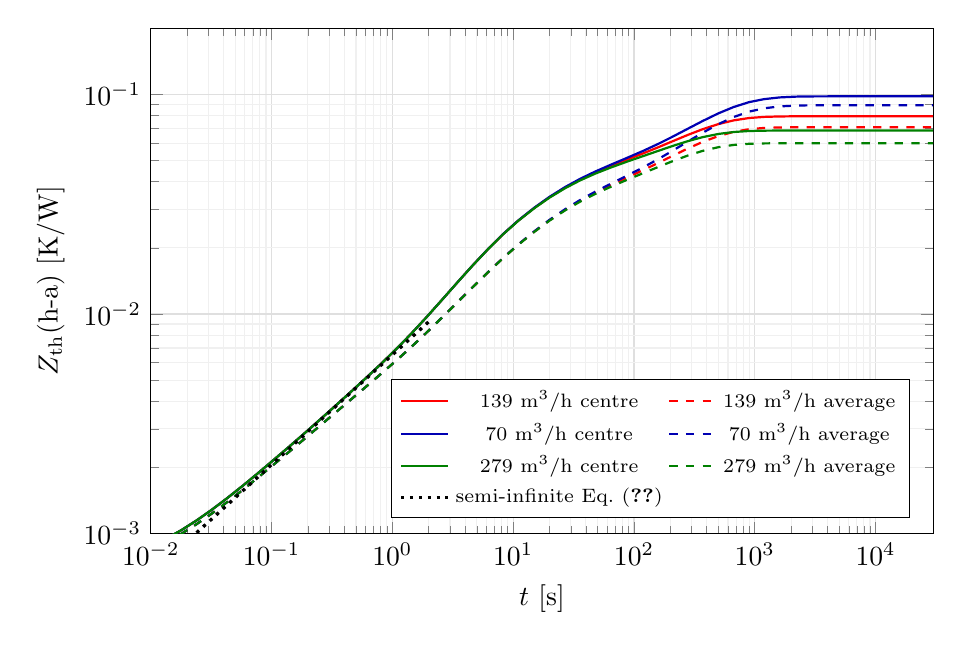
\begin{tikzpicture}
\begin{loglogaxis}[width=0.95\textwidth,height=8cm,xlabel={$t$ [s]},ylabel={$\Zth(\mathrm{h\text{-}a})$ [K/W]},
  grid=both,grid style={gray!25},minor grid style={gray!12},xmin=0.01,xmax=30000,ymin=0.001,ymax=0.2,
  legend style={font=\scriptsize,at={(0.97,0.03)},anchor=south east,legend columns=2}]
\addplot[red,thick] table {
0.01 0.00087576
0.013 0.00093907
0.018 0.0010384
0.024 0.0011487
0.032 0.0012836
0.043 0.0014511
0.058 0.0016543
0.077 0.0018817
0.099 0.0021152
0.139 0.0024798
0.189 0.0028739
0.249 0.0032866
0.339 0.0038246
0.449 0.0043969
0.599 0.0050833
0.799 0.0058985
1.099 0.0070003
1.399 0.0080191
1.899 0.0096091
2.599 0.011657
3.499 0.014031
4.599 0.016587
6.199 0.019752
8.299 0.023148
11 0.026581
15 0.030422
20 0.034013
27 0.03766
36 0.040977
48 0.044103
65 0.04727
87 0.050344
120 0.053939
160 0.057516
210 0.061237
280 0.065395
370 0.069375
500 0.073225
670 0.076139
900 0.078048
1200 0.078955
1600 0.079331
2200 0.079455
2900 0.079474
3900 0.079476
5200 0.079476
7000 0.079476
9300 0.079476
1.2e+04 0.079476
1.7e+04 0.079476
2.2e+04 0.079476
3e+04 0.079476
};
\addplot[red,thick,dashed] table {
0.01 0.00084377
0.013 0.00090448
0.018 0.00099954
0.024 0.001105
0.032 0.0012335
0.043 0.0013924
0.058 0.0015843
0.077 0.0017978
0.099 0.0020156
0.139 0.0023521
0.189 0.0027115
0.249 0.003083
0.339 0.0035598
0.449 0.0040572
0.599 0.0046407
0.799 0.0053158
1.099 0.006198
1.399 0.0069863
1.899 0.00818
2.599 0.0096736
3.499 0.011375
4.599 0.013204
6.199 0.015499
8.299 0.018027
11 0.020672
15 0.023746
20 0.026724
27 0.029856
36 0.032808
48 0.035687
65 0.038696
87 0.041691
120 0.045255
160 0.048828
210 0.052555
280 0.056723
370 0.060715
500 0.064575
670 0.067497
900 0.069412
1200 0.070321
1600 0.070697
2200 0.070822
2900 0.070841
3900 0.070843
5200 0.070843
7000 0.070843
9300 0.070843
1.2e+04 0.070843
1.7e+04 0.070843
2.2e+04 0.070843
3e+04 0.070843
};
\addplot[blue!70!black,thick] table {
0.01 0.00087576
0.013 0.00093907
0.018 0.0010384
0.024 0.0011487
0.032 0.0012836
0.043 0.0014511
0.058 0.0016543
0.077 0.0018817
0.099 0.0021152
0.139 0.0024798
0.189 0.0028739
0.249 0.0032866
0.339 0.0038246
0.449 0.0043969
0.599 0.0050833
0.799 0.0058985
1.099 0.0070003
1.399 0.0080192
1.899 0.0096096
2.599 0.011659
3.499 0.014034
4.599 0.016594
6.199 0.019766
8.299 0.023174
11 0.026628
15 0.030505
20 0.034147
27 0.037871
36 0.041291
48 0.044558
65 0.047931
87 0.05129
120 0.055366
160 0.059607
210 0.064249
280 0.069795
370 0.075599
500 0.081934
670 0.087588
900 0.092194
1200 0.095128
1600 0.096809
2200 0.097638
2900 0.097859
3900 0.097908
5200 0.097913
7000 0.097913
9300 0.097913
1.2e+04 0.097913
1.7e+04 0.097913
2.2e+04 0.097913
3e+04 0.097913
};
\addplot[blue!70!black,thick,dashed] table {
0.01 0.00084377
0.013 0.00090448
0.018 0.00099954
0.024 0.001105
0.032 0.0012335
0.043 0.0013924
0.058 0.0015843
0.077 0.0017978
0.099 0.0020156
0.139 0.0023521
0.189 0.0027115
0.249 0.003083
0.339 0.0035598
0.449 0.0040572
0.599 0.0046407
0.799 0.0053158
1.099 0.0061981
1.399 0.0069865
1.899 0.0081804
2.599 0.0096747
3.499 0.011377
4.599 0.013209
6.199 0.015509
8.299 0.018046
11 0.020707
15 0.023809
20 0.026829
27 0.030027
36 0.03307
48 0.036078
65 0.039282
87 0.042552
120 0.046591
160 0.050824
210 0.05547
280 0.061025
370 0.06684
500 0.073187
670 0.078852
900 0.083466
1200 0.086406
1600 0.08809
2200 0.08892
2900 0.089141
3900 0.089191
5200 0.089196
7000 0.089196
9300 0.089196
1.2e+04 0.089196
1.7e+04 0.089196
2.2e+04 0.089196
3e+04 0.089196
};
\addplot[green!50!black,thick] table {
0.01 0.00087576
0.013 0.00093907
0.018 0.0010384
0.024 0.0011487
0.032 0.0012836
0.043 0.0014511
0.058 0.0016543
0.077 0.0018817
0.099 0.0021152
0.139 0.0024798
0.189 0.0028739
0.249 0.0032866
0.339 0.0038246
0.449 0.0043969
0.599 0.0050833
0.799 0.0058984
1.099 0.0070002
1.399 0.0080189
1.899 0.0096085
2.599 0.011656
3.499 0.014027
4.599 0.016579
6.199 0.019736
8.299 0.023117
11 0.026527
15 0.030326
20 0.033859
27 0.037419
36 0.04062
48 0.043592
65 0.046537
87 0.049312
120 0.052424
160 0.055366
210 0.058255
280 0.061246
370 0.063835
500 0.06602
670 0.067392
900 0.068097
1200 0.068338
1600 0.06841
2200 0.068425
2900 0.068426
3900 0.068426
5200 0.068426
7000 0.068426
9300 0.068426
1.2e+04 0.068426
1.7e+04 0.068426
2.2e+04 0.068426
3e+04 0.068426
};
\addplot[green!50!black,thick,dashed] table {
0.01 0.00084377
0.013 0.00090448
0.018 0.00099954
0.024 0.001105
0.032 0.0012335
0.043 0.0013924
0.058 0.0015843
0.077 0.0017978
0.099 0.0020156
0.139 0.0023521
0.189 0.0027115
0.249 0.003083
0.339 0.0035598
0.449 0.0040572
0.599 0.0046407
0.799 0.0053158
1.099 0.006198
1.399 0.0069862
1.899 0.0081795
2.599 0.0096724
3.499 0.011372
4.599 0.013198
6.199 0.015487
8.299 0.018005
11 0.020632
15 0.023673
20 0.026603
27 0.029661
36 0.032511
48 0.035247
65 0.038047
87 0.040753
120 0.04384
160 0.046782
210 0.049677
280 0.052679
370 0.055278
500 0.057471
670 0.058849
900 0.059556
1200 0.059799
1600 0.05987
2200 0.059886
2900 0.059887
3900 0.059887
5200 0.059887
7000 0.059887
9300 0.059887
1.2e+04 0.059887
1.7e+04 0.059887
2.2e+04 0.059887
3e+04 0.059887
};
\addplot[black,dotted,very thick] table {
0.01 0.0006517
0.02131 0.00095133
0.04541 0.0013887
0.09676 0.0020272
0.2062 0.0029593
0.4394 0.0043199
0.9363 0.0063061
1.995 0.0092055
};
\legend{139 m$^3$/h centre,139 m$^3$/h average,70 m$^3$/h centre,70 m$^3$/h average,279 m$^3$/h centre,279 m$^3$/h average,semi-infinite Eq.~\eqref{eq:semi}}
\end{loglogaxis}
\end{tikzpicture}
\caption{Transient thermal impedance heatsink-to-inlet-air (step response, finite-difference model).}
\label{fig:zth}
\end{figure}

\begin{table}[htbp]
\centering\small
\caption{$\Zth(\mathrm{h\text{-}a})$ in \si{\milli\kelvin\per\watt} at selected times (FD model).}
\label{tab:zth}
\begin{tabular}{r rr rr rr}
\toprule
 & \multicolumn{2}{c}{\SI{70}{\cubic\metre\per\hour}} & \multicolumn{2}{c}{\SI{139}{\cubic\metre\per\hour}} & \multicolumn{2}{c}{\SI{279}{\cubic\metre\per\hour}} \\
\cmidrule(lr){2-3}\cmidrule(lr){4-5}\cmidrule(lr){6-7}
$t$ [s] & avg & centre & avg & centre & avg & centre \\
\midrule
0.1 & 2.0 & 2.1 & 2.0 & 2.1 & 2.0 & 2.1 \\
0.3 & 3.4 & 3.6 & 3.4 & 3.6 & 3.4 & 3.6 \\
1 & 5.9 & 6.6 & 5.9 & 6.6 & 5.9 & 6.6 \\
3 & 10.5 & 12.7 & 10.5 & 12.7 & 10.5 & 12.7 \\
10 & 19.8 & 25.5 & 19.8 & 25.4 & 19.7 & 25.4 \\
30 & 31.1 & 39.1 & 30.9 & 38.9 & 30.7 & 38.6 \\
100 & 44.2 & 53.0 & 43.2 & 51.9 & 42.1 & 50.7 \\
300 & 62.4 & 71.2 & 57.7 & 66.4 & 53.4 & 61.9 \\
1000 & 84.8 & 93.5 & 69.9 & 78.5 & 59.7 & 68.2 \\
3000 & 89.2 & 97.9 & 70.8 & 79.5 & 59.9 & 68.4 \\
\bottomrule
\end{tabular}
\end{table}

\subsection{Foster network}

For circuit or system simulation the curves were fitted from \SI{50}{\milli\second} upwards with four Foster cells,
\begin{equation}
\Zth(t)=\sum_{i=1}^{4} R_i\left(1-e^{-t/\tau_i}\right),\qquad C_i=\tau_i/R_i ,
\end{equation}
Table~\ref{tab:foster} (maximum deviation \SI{5}{\percent} of the local value, \SI{1.4}{\percent} of the final value). The first three cells are practically flow independent; only $R_4$ and $\tau_4$ change with $Q$. For a flow other than the tabulated ones, keep cells 1--3 of the \SI{139}{\cubic\metre\per\hour} set and take $R_4=\Rth(Q)-R_1-R_2-R_3$ with $\tau_4\approx 6.0\,\si{\kilo\joule\per\kelvin}\cdot R_4$.

\begin{table}[htbp]
\centering\small
\caption{Four-cell Foster parameters of $\Zth(\mathrm{h\text{-}a})$. $R_i$ in \si{\milli\kelvin\per\watt}, $\tau_i$ in \si{\second}, $C_i$ in \si{\joule\per\kelvin}.}
\label{tab:foster}
\begin{tabular}{c rrr rrr}
\toprule
 & \multicolumn{3}{c}{contact-area average} & \multicolumn{3}{c}{contact-area centre} \\
\cmidrule(lr){2-4}\cmidrule(lr){5-7}
$i$ & $R_i$ & $\tau_i$ & $C_i$ & $R_i$ & $\tau_i$ & $C_i$ \\
\midrule
\multicolumn{7}{l}{\emph{$Q=\SI{70}{\cubic\metre\per\hour}$ ($V_{ch}=\SI{2}{\metre\per\second}$)}}\\
1 & 1.65 & 0.04 & 27 & 1.74 & 0.05 & 27 \\
2 & 3.27 & 0.79 & 240 & 3.09 & 0.86 & 278 \\
3 & 24.68 & 12.89 & 522 & 33.04 & 11.59 & 351 \\
4 & 59.49 & 371.55 & 6246 & 59.91 & 366.32 & 6114 \\
\midrule
$\sum R_i$ & 89.1 & & & 97.8 & & \\
\midrule
\multicolumn{7}{l}{\emph{$Q=\SI{139}{\cubic\metre\per\hour}$ ($V_{ch}=\SI{4}{\metre\per\second}$)}}\\
1 & 1.61 & 0.04 & 27 & 1.63 & 0.04 & 26 \\
2 & 3.14 & 0.73 & 232 & 2.69 & 0.67 & 249 \\
3 & 24.18 & 12.31 & 509 & 32.51 & 10.85 & 334 \\
4 & 41.81 & 250.64 & 5995 & 42.51 & 242.93 & 5715 \\
\midrule
$\sum R_i$ & 70.7 & & & 79.3 & & \\
\midrule
\multicolumn{7}{l}{\emph{$Q=\SI{279}{\cubic\metre\per\hour}$ ($V_{ch}=\SI{8}{\metre\per\second}$)}}\\
1 & 1.56 & 0.04 & 26 & 1.47 & 0.04 & 25 \\
2 & 2.97 & 0.66 & 221 & 2.37 & 0.49 & 208 \\
3 & 23.45 & 11.58 & 494 & 31.46 & 10.00 & 318 \\
4 & 31.80 & 176.97 & 5564 & 32.97 & 166.10 & 5037 \\
\midrule
$\sum R_i$ & 59.8 & & & 68.3 & & \\
\bottomrule
\end{tabular}
\end{table}

\subsection{Use with the device data}

The junction temperature follows from the series chain
\begin{equation}
T_j(t) = T_{air,in} + P * \left[\Zth(\mathrm{j\text{-}c}) + \Rth(\mathrm{c\text{-}h}) + \Zth(\mathrm{h\text{-}a})\right],
\end{equation}
where $\Zth(\mathrm{j\text{-}c})$ and the contact resistance $\Rth(\mathrm{c\text{-}h})$ (single-side cooled value) are taken from the thyristor datasheet and $*$ denotes convolution. For a device with a \O\,\SI{100}{\milli\metre} pole face $\Rth(\mathrm{c\text{-}h})$ is typically \SIrange{3}{5}{\milli\kelvin\per\watt} per side, i.e.\ small compared with the heatsink. If two devices are mounted, one on each face, each device sees approximately the half-heatsink (fins with adiabatic mid-plane); the per-device resistance is then about 1.4--1.6 times the values given here (analytical estimate, higher factor at low flow) rather than twice, because the spreading resistance does not double.

\section{Summary}\label{sec:summary}

\begin{table}[htbp]
\centering\small
\caption{Proposed design values for heatsink 778746, single device, contact-face centre, including \SI{15}{\percent} margin on the finite-difference result.}
\label{tab:summary}
\begin{tabular}{rrrrr}
\toprule
$Q$ [\si{\cubic\metre\per\hour}] & $V_{ch}$ [\si{\metre\per\second}] & $\Delta p$ [\si{\pascal}] & $\Rth^{max}$ FD [\si{\kelvin\per\watt}] & design $\Rth(\mathrm{h\text{-}a})$ [\si{\kelvin\per\watt}] \\
\midrule
 70 & 2 & 11 & 0.098 & 0.113 \\
104 & 3 & 18 & 0.086 & 0.099 \\
139 & 4 & 28 & 0.080 & 0.091 \\
209 & 6 & 53 & 0.073 & 0.083 \\
279 & 8 & 84 & 0.068 & 0.079 \\
\bottomrule
\end{tabular}
\end{table}

\begin{itemize}
\item The heatsink is a closed-channel forced-air design; usable performance requires a fan delivering \SIrange{100}{300}{\cubic\metre\per\hour} \emph{through} the heatsink at \SIrange{20}{90}{\pascal}.
\item The resistance is split roughly half and half between plate spreading (flow independent, about \SI{0.04}{\kelvin\per\watt} at the centre) and convection. Above \SI{200}{\cubic\metre\per\hour} the return on additional flow is small.
\item With a \SI{60}{\kelvin} allowed rise above inlet air, the dissipable power is about \SIrange{650}{750}{\watt} per heatsink in the \SIrange{140}{280}{\cubic\metre\per\hour} range.
\item For overloads shorter than about \SI{30}{\second} the transient impedance does not depend on the flow; the Foster set of Table~\ref{tab:foster} can be used directly.
\item The estimate should be confirmed by a measurement on a sample or by manufacturer data for the profile ``G'' assembly, in particular for the behaviour of the module joints.
\end{itemize}

\begin{thebibliography}{9}
\bibitem{teertstra1999} P.~Teertstra, M.~M. Yovanovich, J.~R. Culham, ``Analytical forced convection modeling of plate fin heat sinks,'' \emph{Proc.\ 15th IEEE SEMI-THERM Symposium}, San Diego, 1999, pp.~34--41.
\bibitem{lee1995} S.~Lee, S.~Song, V.~Au, K.~P. Moran, ``Constriction/spreading resistance model for electronics packaging,'' \emph{Proc.\ 4th ASME/JSME Thermal Engineering Joint Conference}, vol.~4, 1995, pp.~199--206.
\bibitem{shah1978} R.~K. Shah, A.~L. London, \emph{Laminar Flow Forced Convection in Ducts}, Academic Press, New York, 1978.
\bibitem{kays1984} W.~M. Kays, A.~L. London, \emph{Compact Heat Exchangers}, 3rd ed., McGraw-Hill, 1984.
\bibitem{elenbaas1942} W.~Elenbaas, ``Heat dissipation of parallel plates by free convection,'' \emph{Physica}, vol.~9, no.~1, 1942, pp.~1--28.
\bibitem{incropera} F.~P. Incropera, D.~P. DeWitt, T.~L. Bergman, A.~S. Lavine, \emph{Fundamentals of Heat and Mass Transfer}, 6th ed., Wiley, 2007 (extended surfaces, Ch.~3).
\bibitem{simons2004} R.~E. Simons, ``Simple formulas for estimating thermal spreading resistance,'' \emph{Electronics Cooling}, May 2004.
\end{thebibliography}

\appendix
\section{Analytical model script}\label{app:analytic}
Python~3 with NumPy; reproduces Table~\ref{tab:sweep} (analytical columns).
\begin{lstlisting}
"""
Heatsink 778746 (SECOM, PADA profile "G", L = 250 mm) -- analytical steady-state model.
Forced convection through the internal channels, fin analysis, Lee spreading resistance,
pressure drop. Reproduces Table 3 of the accompanying note.
"""
import numpy as np

# ---- geometry [m] (from drawing 778746-01-01) ----
W, Hs, L = 0.225, 0.091, 0.250      # width across fins, height, length (flow direction)
tb   = 0.014                        # base plate thickness, each side (surface to fin root)
tf   = 0.0016                       # fin (web) thickness
b    = 0.00415                      # channel width
Nf, Nch = 36, 37                    # fins, channels
tw   = (W - Nf*tf - Nch*b)/2        # side wall thickness (~6.9 mm)
Lf   = Hs - 2*tb                    # fin length plate to plate (63 mm)
Ds   = 0.100                        # SCR contact diameter
a    = Ds/2; As = np.pi*a**2; Ap = W*L; rp = np.sqrt(Ap/np.pi)

# ---- materials ----
k = 200.0                           # Al 6060/6063 extrusion [W/(m K)]
rho_a, cp_a, k_a, nu_a, Pr = 1.127, 1007.0, 0.0271, 1.70e-5, 0.71   # air, 40 degC

Aff  = Nch*b*Lf                     # free flow area
Afr  = W*Hs
sigma = Aff/Afr
Dh   = 2*b*Lf/(b+Lf)
Atop = Nch*b*L                      # channel top walls (at base temperature)

def h_channel(Vch):
    """Teertstra, Yovanovich, Culham (1999), h referred to inlet air temperature."""
    Reb = Vch*b/nu_a
    Res = Reb*b/L
    nu_fd  = Res*Pr/2
    nu_dev = 0.664*np.sqrt(Res)*Pr**(1/3)*np.sqrt(1 + 3.65/np.sqrt(Res))
    Nu = (nu_fd**-3 + nu_dev**-3)**(-1/3)
    return Nu*k_a/b, Nu, Reb, Res

def fin_conductance(h, t, two_sided, tip_ratio):
    """Conductance [W/K] of one fin (thickness t, length Lf, depth L) whose tip is
    attached to the bottom plate; the plate is modelled as a convective tip with
    h_t = h*tip_ratio (tip_ratio = collector area / fin cross-section)."""
    P  = 2*L if two_sided else L
    Ac = t*L
    m  = np.sqrt(h*P/(k*Ac));  M = np.sqrt(h*P*k*Ac)
    z  = h*tip_ratio/(m*k);   mL = m*Lf
    G  = M*(np.sinh(mL) + z*np.cosh(mL))/(np.cosh(mL) + z*np.sinh(mL))
    return G, mL

def G_total(h):
    Gf, mL = fin_conductance(h, tf, True,  b/tf)        # internal fins
    Gw, _  = fin_conductance(h, tw, False, (b/2)/tw)    # side walls, inner face only
    G = Nf*Gf + 2*Gw + h*Atop
    eta_eff = Gf/(h*2*Lf*L)
    return G, mL, eta_eff

def lee_spreading(heff, kk=k):
    """Lee, Song, Au, Moran (1995): circular source (radius a) on a circular plate
    (radius rp, thickness tb) with uniform h_eff on the back. Returns R_max, R_avg, R_1D."""
    eps, tau, Bi = a/rp, tb/rp, heff*rp/kk
    lam = np.pi + 1/(eps*np.sqrt(np.pi))
    Phi = (np.tanh(lam*tau) + lam/Bi)/(1 + lam/Bi*np.tanh(lam*tau))
    psi_max = eps*tau/np.sqrt(np.pi) + (1-eps)*Phi/np.sqrt(np.pi)
    psi_avg = eps*tau/np.sqrt(np.pi) + 0.5*(1-eps)**1.5*Phi
    return psi_max/(kk*np.sqrt(As)), psi_avg/(kk*np.sqrt(As)), tb/(kk*Ap)

def pressure_drop(Vch):
    """Laminar developing flow in a rectangular duct (Shah & London) + contraction/expansion."""
    Re = Vch*Dh/nu_a
    al = b/Lf
    fRe = 24*(1 - 1.3553*al + 1.9467*al**2 - 1.7012*al**3 + 0.9564*al**4 - 0.2537*al**5)  # Fanning
    xp = L/(Dh*Re)
    fapp = (3.44/np.sqrt(xp) + (fRe + 0.674/(4*xp) - 3.44/np.sqrt(xp))/(1 + 2.9e-5/xp**2))/Re
    Kc, Ke = 0.42*(1 - sigma**2), (1 - sigma**2)**2
    return 0.5*rho_a*Vch**2*(4*fapp*L/Dh + Kc + Ke)

if __name__ == "__main__":
    print(f"Lf={Lf*1e3:.0f} mm  tw={tw*1e3:.1f} mm  Aff={Aff*1e4:.1f} cm2  sigma={sigma:.3f}  Dh={Dh*1e3:.2f} mm  rp={rp*1e3:.1f} mm")
    print(" Q[m3/h] Vch[m/s]  Re_b  Nu_b  h[W/m2K] eta_f  G[W/K]  R_conv  R_sp,avg R_sp,max R_th,avg R_th,max dp[Pa]")
    for Vch in [1, 1.5, 2, 2.5, 3, 4, 5, 6, 7, 8, 10]:
        h, Nu, Reb, Res = h_channel(Vch)
        G, mL, eta = G_total(h)
        Rmax, Ravg, R1d = lee_spreading(G/Ap)
        Q = Vch*Aff*3600
        print(f"{Q:7.0f} {Vch:7.1f} {Reb:6.0f} {Nu:5.2f} {h:8.1f} {eta:6.3f} {G:7.2f} {1/G:8.4f} {Ravg:8.4f} {Rmax:8.4f} {1/G+Ravg:8.4f} {1/G+Rmax:8.4f} {pressure_drop(Vch):6.1f}")
\end{lstlisting}

\section{Finite-difference model script}\label{app:fd}
Requires NumPy and SciPy; imports the file above. Run time about three minutes.
\begin{lstlisting}
"""
Heatsink 778746 -- 3-D finite-difference thermal model (steady state and step response).
Top plate: 3-D (x, y, z); fins and side walls: 2-D (x, s); bottom plate: 3-D (x, y, z).
Uniform channel h from hs778746_analytic.h_channel, referred to inlet air temperature.
Run:  python hs778746_fd.py   (about 3 min; writes results_fd.json and foster.json)
"""
import json, time
import numpy as np
import scipy.sparse as sp
import scipy.sparse.linalg as spla
from scipy.optimize import curve_fit
from hs778746_analytic import (W, Hs, L, tb, tf, b, Nf, tw, Lf, a, Ap, As, Aff, k,
                               h_channel, G_total, lee_spreading, pressure_drop)
rho, cp = 2700.0, 900.0

def build(h, hj=np.inf, Nx=50, Nz=7, Ns=10, Nzb=2, h_out=0.0):
    """Assemble conductance matrix K, capacitance vector C and unit-power vector P."""
    dx = L/Nx
    p  = tf + b
    we = tw + b/2                              # edge cell: side wall + half channel
    wy = np.array([we] + [p]*Nf + [we]); Ny = len(wy)
    dz, ds, dzb = tb/Nz, Lf/Ns, tb/Nzb
    n = 0
    itp = np.arange(Nx*Ny*Nz).reshape(Nx, Ny, Nz);      n += itp.size
    ifn = n + np.arange(Nx*Nf*Ns).reshape(Nx, Nf, Ns);  n += ifn.size
    iwl = n + np.arange(Nx*2*Ns).reshape(Nx, 2, Ns);    n += iwl.size
    ibp = n + np.arange(Nx*Ny*Nzb).reshape(Nx, Ny, Nzb); n += ibp.size
    N = n
    C = np.zeros(N); Gg = np.zeros(N); I = []; J = []; V = []
    link = lambda i, j, g: (I.append(i), J.append(j), V.append(g))
    # plates
    for idx, nz, dzz in ((itp, Nz, dz), (ibp, Nzb, dzb)):
        for ix in range(Nx):
            for iy in range(Ny):
                for iz in range(nz):
                    nd = idx[ix, iy, iz]
                    C[nd] = rho*cp*dx*wy[iy]*dzz
                    if ix+1 < Nx: link(nd, idx[ix+1, iy, iz], k*wy[iy]*dzz/dx)
                    if iy+1 < Ny:
                        g = k*dx*dzz/(0.5*(wy[iy]+wy[iy+1]))
                        if 1 <= iy <= Nf-1 and iy % 2 == 0 and np.isfinite(hj):   # module joint every 2 fins
                            g = 1/(1/g + 1/(hj*dx*dzz))
                        link(nd, idx[ix, iy+1, iz], g)
                    if iz+1 < nz: link(nd, idx[ix, iy, iz+1], k*dx*wy[iy]/dzz)
    # fins
    for ix in range(Nx):
        for jf in range(Nf):
            iy = jf + 1
            for s in range(Ns):
                nd = ifn[ix, jf, s]
                C[nd] = rho*cp*dx*tf*ds
                Gg[nd] += h*2*dx*ds
                if ix+1 < Nx: link(nd, ifn[ix+1, jf, s], k*tf*ds/dx)
                if s+1 < Ns:  link(nd, ifn[ix, jf, s+1], k*dx*tf/ds)
            link(ifn[ix, jf, 0],    itp[ix, iy, Nz-1], 1/((dz/2)/(k*dx*wy[iy]) + (ds/2)/(k*dx*tf)))
            link(ifn[ix, jf, Ns-1], ibp[ix, iy, 0],    1/((dzb/2)/(k*dx*wy[iy]) + (ds/2)/(k*dx*tf)))
            Gg[itp[ix, iy, Nz-1]] += h*dx*(wy[iy]-tf)      # channel top wall
            Gg[ibp[ix, iy, 0]]    += h*dx*(wy[iy]-tf)      # channel bottom wall
    # side walls (inner face convects)
    for ix in range(Nx):
        for jw, iy in enumerate((0, Ny-1)):
            for s in range(Ns):
                nd = iwl[ix, jw, s]
                C[nd] = rho*cp*dx*tw*ds
                Gg[nd] += h*dx*ds + h_out*dx*ds
                if ix+1 < Nx: link(nd, iwl[ix+1, jw, s], k*tw*ds/dx)
                if s+1 < Ns:  link(nd, iwl[ix, jw, s+1], k*dx*tw/ds)
            link(iwl[ix, jw, 0],    itp[ix, iy, Nz-1], 1/((dz/2)/(k*dx*wy[iy]) + (ds/2)/(k*dx*tw)))
            link(iwl[ix, jw, Ns-1], ibp[ix, iy, 0],    1/((dzb/2)/(k*dx*wy[iy]) + (ds/2)/(k*dx*tw)))
            Gg[itp[ix, iy, Nz-1]] += h*dx*(wy[iy]-tw)
            Gg[ibp[ix, iy, 0]]    += h*dx*(wy[iy]-tw)
    if h_out > 0:                                          # optional: outer face of bottom plate
        for ix in range(Nx):
            for iy in range(Ny):
                Gg[ibp[ix, iy, Nzb-1]] += h_out*dx*wy[iy]
    I, J, V = map(np.array, (I, J, V))
    K = sp.coo_matrix((np.r_[V, V, -V, -V], (np.r_[I, J, I, J], np.r_[I, J, J, I])), shape=(N, N)).tocsr()
    K = K + sp.diags(Gg)
    # source: fraction of each top cell inside the circle of radius a
    xc = (np.arange(Nx)+0.5)*dx - L/2
    ye = np.r_[0, np.cumsum(wy)] - W/2
    frac = np.zeros((Nx, Ny)); sub = 8
    for ix in range(Nx):
        xs = xc[ix] - dx/2 + (np.arange(sub)+0.5)*dx/sub
        for iy in range(Ny):
            ys = ye[iy] + (np.arange(sub)+0.5)*wy[iy]/sub
            X, Y = np.meshgrid(xs, ys)
            frac[ix, iy] = np.mean(X**2 + Y**2 <= a**2)
    Acell = dx*wy[None, :]*frac
    P = np.zeros(N); P[itp[:, :, 0].ravel()] = (Acell/Acell.sum()).ravel()
    q = P[itp[:, :, 0]]/(dx*wy[None, :])                    # flux per unit power
    geom = dict(itp=itp, ifn=ifn, iwl=iwl, ibp=ibp, Acell=Acell, q=q, dz=dz,
                xc=xc, yc=np.cumsum(wy)-wy/2-W/2, frac=frac, N=N, Gg=Gg)
    return K, C, P, geom

def surface(T, geom):
    """Contact-face temperature per unit power: node value + half-cell correction."""
    return T[geom['itp'][:, :, 0]] + geom['q']*(geom['dz']/2)/k

def steady(K, P, geom):
    T = spla.spsolve(K.tocsc(), P)
    Ts = surface(T, geom); A = geom['Acell']
    return T, Ts, (Ts*A).sum()/A.sum(), Ts[A > 0].max()

def transient(K, C, P, geom, decades=(-3, 5), spd=90):
    """Implicit Euler step response; constant dt inside each decade (spd steps per decade)."""
    N = len(C); T = np.zeros(N); t = 0.0; Cd = sp.diags(C); A = geom['Acell']
    ts, Za, Zm = [], [], []
    for dec in range(*decades):
        dt = 10.0**dec/(spd/9)
        lu = spla.splu((Cd/dt + K).tocsc())
        for _ in range(spd):
            T = lu.solve(C*T/dt + P); t += dt
            Ts = surface(T, geom)
            ts.append(t); Za.append((Ts*A).sum()/A.sum()); Zm.append(Ts[A > 0].max())
    return np.array(ts), np.array(Za), np.array(Zm)

def foster_fit(t, Z, n=4, tmin=0.05):
    f = lambda t, *p: sum(np.exp(p[i])*(1-np.exp(-t/np.exp(p[n+i]))) for i in range(n))
    m = t >= tmin
    p0 = np.r_[np.log(np.full(n, Z[-1]/n)), np.log(np.logspace(-0.5, 2.5, n))]
    popt, _ = curve_fit(f, t[m], Z[m], p0=p0, sigma=Z[m]*0.02 + 2e-5, maxfev=40000)
    R, tau = np.exp(popt[:n]), np.exp(popt[n:]); o = np.argsort(tau)
    return R[o], tau[o], np.max(np.abs(f(t[m], *popt) - Z[m])/Z[m])

if __name__ == "__main__":
    out = {'sweep': [], 'joint': [], 'zth': {}}
    for Vch in [1, 1.5, 2, 2.5, 3, 4, 5, 6, 7, 8, 10]:
        h, Nu, Reb, Res = h_channel(Vch)
        K, C, P, geom = build(h)
        T, Ts, Ravg, Rmax = steady(K, P, geom)
        G, mL, eta = G_total(h); Rsm, Rsa, _ = lee_spreading(G/Ap)
        out['sweep'].append(dict(V=Vch, Q=Vch*Aff*3600, Reb=Reb, Nu=Nu, h=h, eta=eta, G=G,
                                 Ran_avg=1/G+Rsa, Ran_max=1/G+Rsm, Rsp_avg=Rsa, Rsp_max=Rsm,
                                 Rfd_avg=Ravg, Rfd_max=Rmax, dp=pressure_drop(Vch)))
        print(f"V={Vch:4.1f} m/s  Q={Vch*Aff*3600:4.0f} m3/h  analytic {1/G+Rsa:.4f}/{1/G+Rsm:.4f}  FD {Ravg:.4f}/{Rmax:.4f} K/W")
    h = h_channel(4.0)[0]
    for hj in [np.inf, 5e4, 2e4, 1e4, 5e3]:
        K, C, P, geom = build(h, hj=hj); _, _, Ravg, Rmax = steady(K, P, geom)
        out['joint'].append(dict(hj=hj, Ravg=Ravg, Rmax=Rmax)); print("joint hj =", hj, Ravg, Rmax)
    K, C, P, geom = build(h, h_out=5.0); _, _, Ravg, Rmax = steady(K, P, geom)
    out['hout5'] = dict(Ravg=Ravg, Rmax=Rmax); print("h_out = 5:", Ravg, Rmax)
    K, C, P, geom = build(h); T, Ts, Ravg, Rmax = steady(K, P, geom)
    itp = geom['itp']; iy0 = np.argmin(np.abs(geom['yc'])); ix0 = np.argmin(np.abs(geom['xc']))
    out['prof_x'] = dict(x=(geom['xc']*1e3).tolist(), Tsurf=Ts[:, iy0].tolist(),
                         Troot=T[itp[:, iy0, -1]].tolist(), Tbot=T[geom['ibp'][:, iy0, 0]].tolist())
    out['prof_y'] = dict(y=(geom['yc']*1e3).tolist(), Tsurf=Ts[ix0, :].tolist(),
                         Troot=T[itp[ix0, :, -1]].tolist(), Tbot=T[geom['ibp'][ix0, :, 0]].tolist())
    Pc = geom['Gg']*T; mask = np.zeros(len(T), bool)
    for ix in range(len(geom['xc'])):
        for jf in range(Nf):
            if geom['frac'][ix, jf+1] > 0.5: mask[geom['ifn'][ix, jf, :]] = True
    out['share_under_source'] = float(Pc[mask].sum()); out['mass'] = float(C.sum()/cp)
    print("mass", out['mass'], "kg; share under footprint", out['share_under_source'])
    fits = {}
    for Vch in [2.0, 4.0, 8.0]:
        h = h_channel(Vch)[0]; K, C, P, geom = build(h); t0 = time.time()
        ts, Za, Zm = transient(K, C, P, geom)
        out['zth'][str(Vch)] = dict(t=ts.tolist(), Zavg=Za.tolist(), Zmax=Zm.tolist())
        for key, Z in (('Zavg', Za), ('Zmax', Zm)):
            R, tau, err = foster_fit(ts, Z)
            fits[f"{Vch}_{key}"] = dict(R=R.tolist(), tau=tau.tolist(), err=float(err))
            print(f"V={Vch} {key}: R_i [mK/W] = {np.round(R*1e3,2)}  tau_i [s] = {np.round(tau,2)}  max rel err {err*100:.1f}%  ({time.time()-t0:.0f} s)")
    json.dump(out, open('results_fd.json', 'w')); json.dump(fits, open('foster.json', 'w'))
\end{lstlisting}

\end{document}
